% Chapter Template
\tocdata{toc}{Di Wan}

\chapter{Recommendation Engine}% Main chapter title
\label{Chapter6} % Change X to a consecutive number; for referencing this chapter elsewhere, use \ref{ChapterX}

\section{Introduction}
A recommendation engine is a data filtering tool using machine learning algorithms to recommend the most relevant items to a particular user or customer. 
It operates on finding patterns in consumer behaviour data, which can be collected implicitly or explicitly.\footfullcite{} In our case, the quality of the recommendation system design determines the quality of the posts recommended to our users.
\\A recent study by Epsilon found that 90\% of consumers find personalisation appealing. A further 80\% claim they are more likely to cooperate with a company when offered personalised experiences.
The study also found that these consumers are ten times more likely to become VIP customers who make more than 15 purchases per year.\footfullcite{epsilon} 
Thus a well-designed recommendation system can benefit the monetisation of our app in the future.
\\Recommendation systems are divided into personalised and non-personalised systems, where personalised recommendation systems can be further divided into content-based and collaborative filtering systems. 
The overview of the recommendation system can be seen in figure \ref{fig:overrecomm}.
\begin{figure}[ht]
\centering
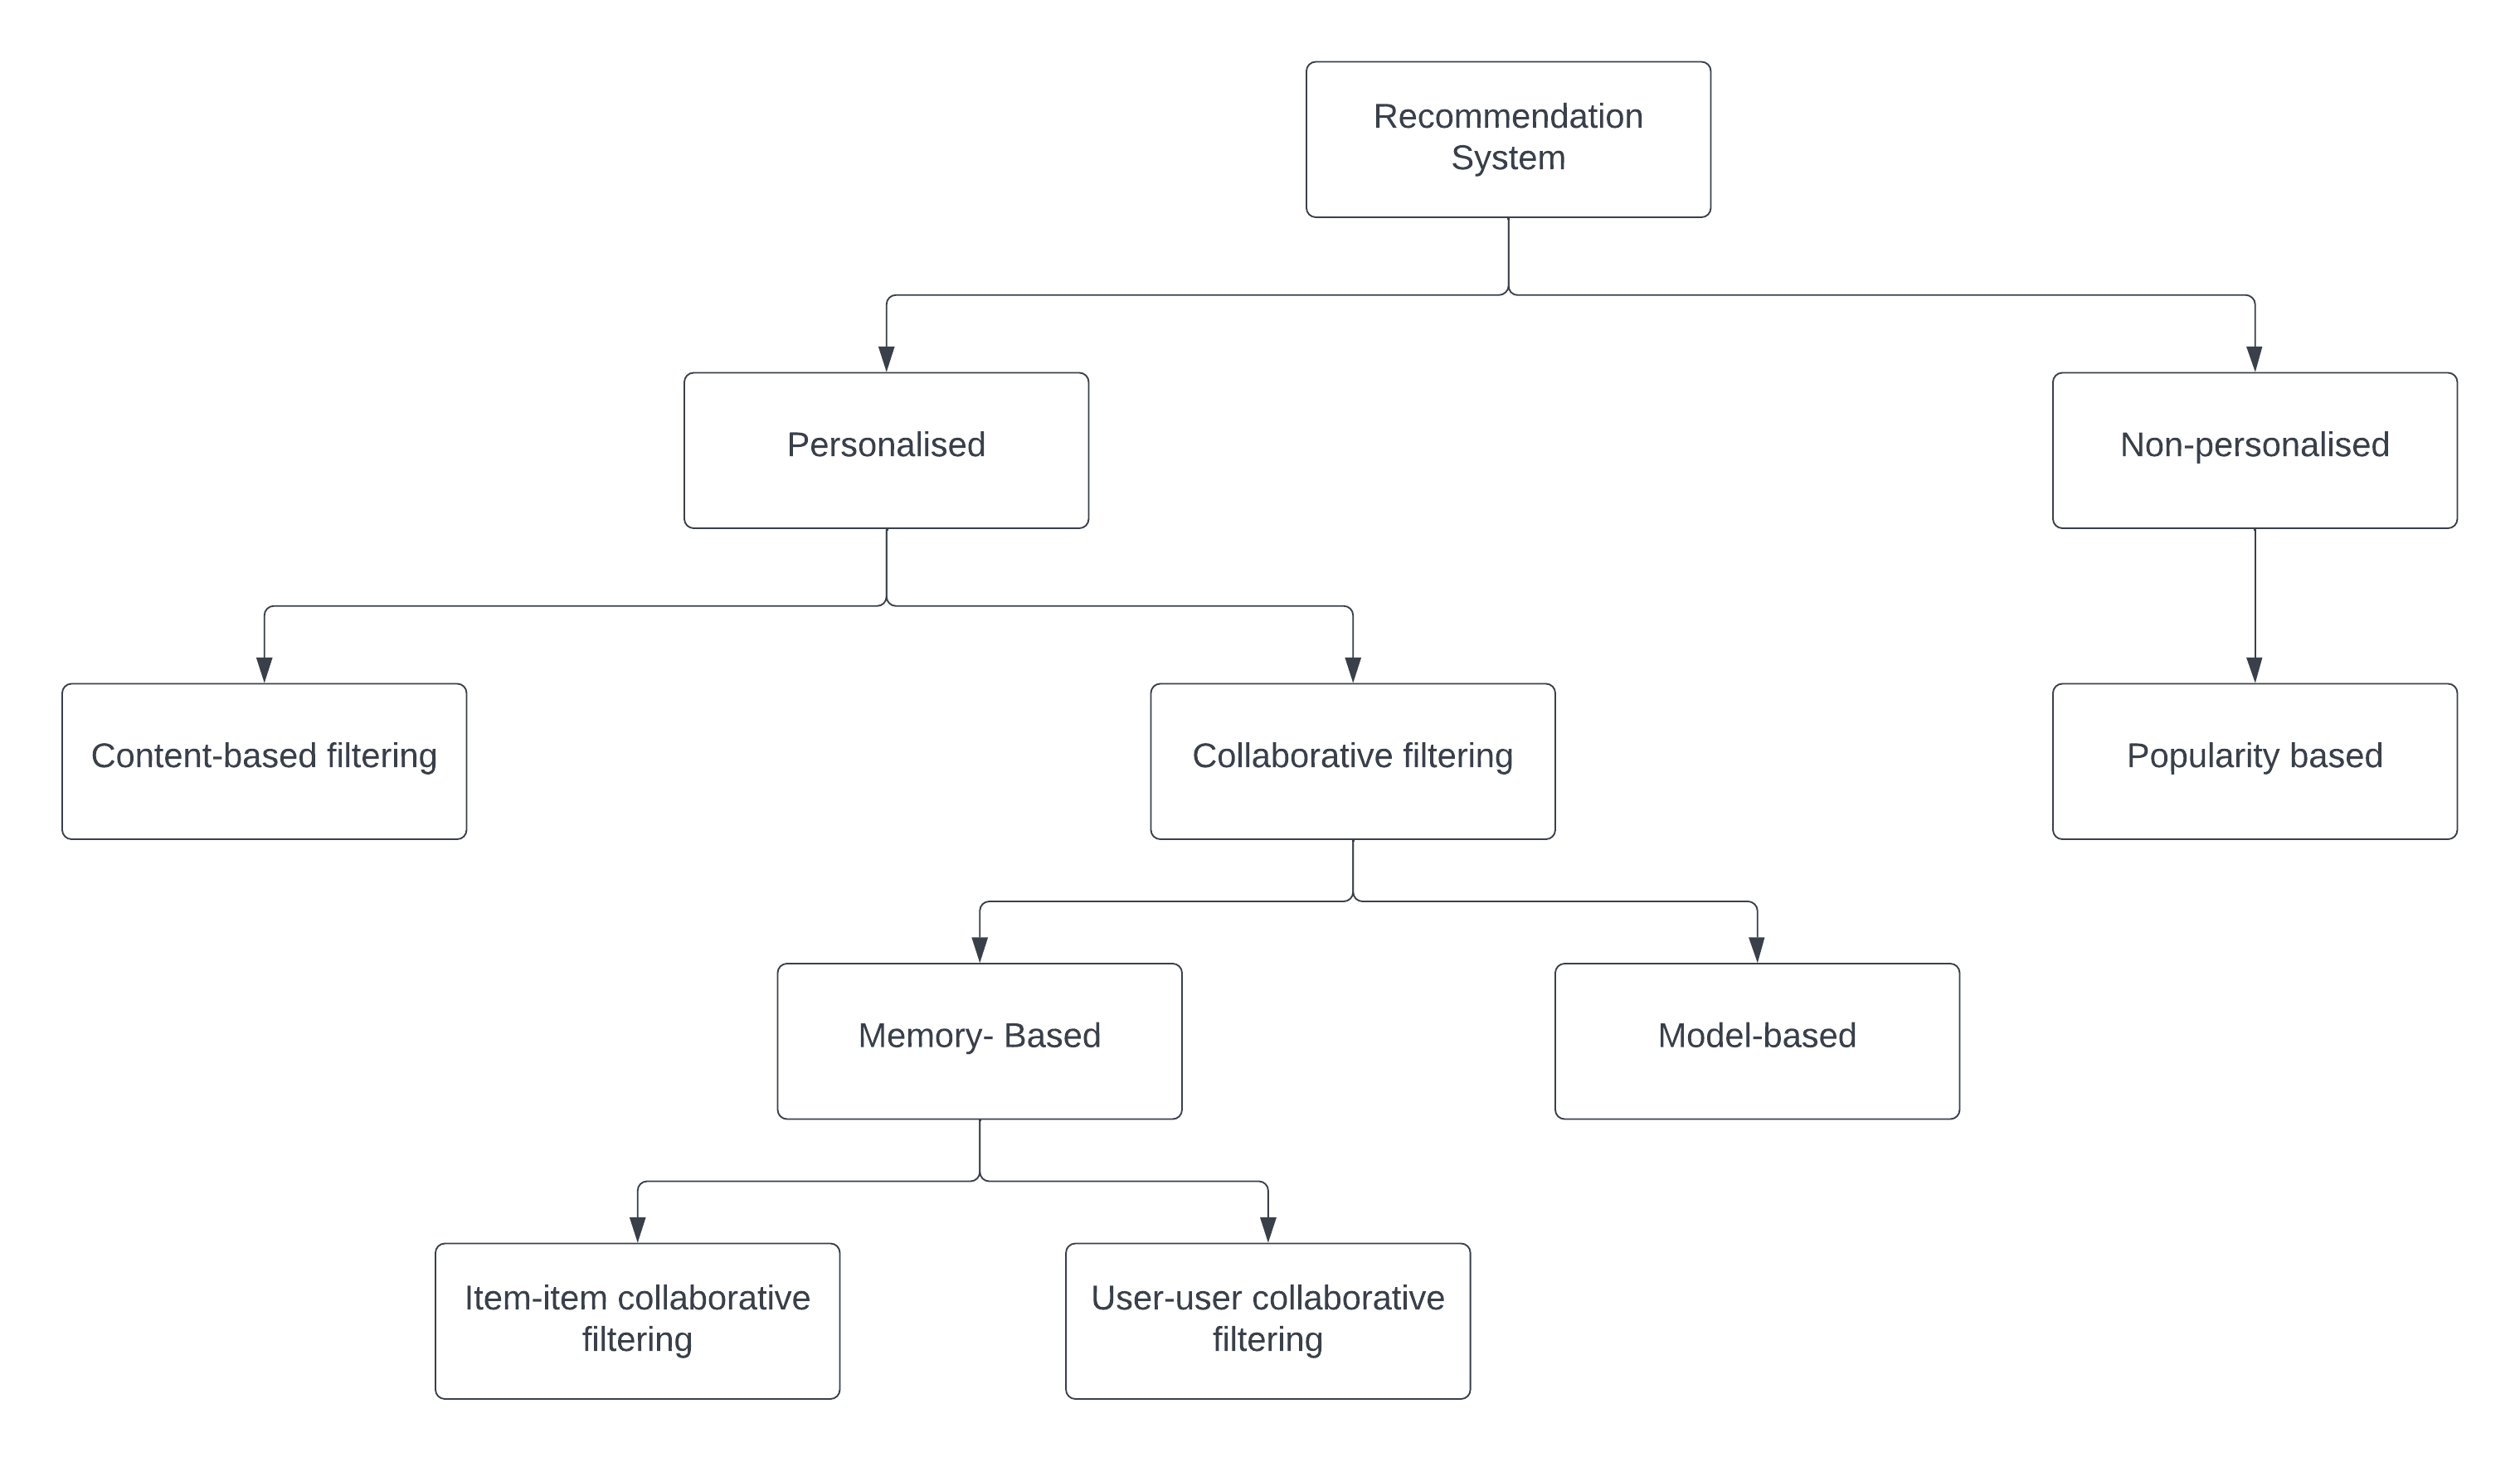
\includegraphics[width=0.8\columnwidth]{overview11.png}
\caption{Overview of recommendation system}
\label{fig:overrecomm}
\end{figure}

%-----------------------------------------------------------------------------------------------------------------------------Popularity-Based Recommendation System
\section{Popularity-based Recommendation System}
Popularity-based recommendation system works on the principle of popularity or anything in trend. These systems check the items in trend or are most popular among the users and directly recommend those. 
For our design, instead of recommending posts only based on the number of likes that the posts received, we can give weighting to each parameter involved in our decision. One of the weighted rating models we constructed is shown below.
\begin{equation*}
\text{Rating} = f(L,C,m,g,T) = \alpha \times \frac{L^{2}}{L+m} + \beta \times \frac{C^{2}}{C+m} + T \times g_{[k-2,k]}
\end{equation*}
Where:
\\$L$ is the number of likes the post received.
\\$C$ is the number of comments the post received.
\\$m$ is the minimum of like preferences required to be listed as a popular item.
\\$g_{[k-2,k]}$ is the gradient of change in the total number of likes and comments in w.r.t time in the last two days, which is calculated by 
$g_{[k-2,k]} = \frac{L_{k} + C_{k} -L_{k-2} -C_{k-2}}{2}$, with $k$ indicates \textit{the current day} and $(k-3)$ indicates \textit{three days ago}.
\\$T$ is the period and we set $T=1$.
\\ $\alpha$ and $\beta$ are constants.
\\This formula is a modified version based on the rating system by IMDB \footfullcite{}, which is an online database of information related to films and television series. We introduced non-linearity in the weightings for $L$ and $C$, and it can be seen that we set a threshold for these two parameters; for example, if $L \gg m$, then the first term on the right-hand side will be dominated by $L$, same for $C$ in the second term. The non-linearity here is to attenuate the contribution brought by $L$ and $C$ when these values are small. The last term on the right-hand side predicts the increase in the total number of likes and comments by assuming the gradient change the day after is the same as two days ago. Further improvement is made by introducing $\alpha$ and $\beta$ to indicate the relative significances of $L$ and $C$, and it is usually considered that $L$ is more significant than $C$. Thus $\alpha > \beta$. Finally, the system will rank the posts by the ratings.
\\The advantage of the popularity based system is that it is easy to implement and requires relatively low computational power. However, the most apparent disadvantage of a popularity-based system is the non-personalisation because it does not analyse the individual user's preference.


%-----------------------------------------------------------------------------------------------------------------------------Content-Based Recommendation System
\section{Content Based Recommendation System}
\label{Content Based Recommendation System}
Content-Based recommendation systems depend on a profile of the user's preferences and feature descriptions of the item.
The recommendation is modelled as a user-specific classification problem that estimates users' likes and dislikes based on an item's features with a content-based recommender.
\\ We assume that there are available features that captures the content of the item.
\\ First we need to obtain the post-feature matrix (Table:\ref{itemfea}).
\begin{table}[ht]
\centering
\begin{tabular}{ |c|c|c|c|c|c|} 
 \hline
 \diagbox{Posts}{Features}&Feature1&Feature 2&Feature 3&$\cdots$&Feature $j$\\
 \hline
 Post1&&&&&\\
 \hline
 Post2&&&&&\\
 \hline
 $\vdots$&&&&&\\
 \hline
 Post $i$&&&&&\\
 \hline
 \end{tabular}
 \caption{Post Feature Matrix}
 \label{itemfea}
 \end{table}
\\The ratings given in the table measures the degree of the features in the posts, and we can assume the matrix is not sparse, which we mean the matrix is fully filled. And we denote that each row is the feature vector $x(i)$ for post $i$.
%
\\In addition, we need to get the profile of each user, which means we need to know and analyse the preferences of our users, 
so we need to obtain the user parameter vector for each user, reflecting how the user responds to the features.
%
\\After we have the post-feature matrix and the user parameter vector $\theta(j)$ of user $j$, we apply similarity metrics, and we use cosine similarity to measure the resonance between $\theta(j)$ and each $x(i)$ in the post-feature matrix.
\\Cosine Similarity,  as the name mentioned, it measures the cosine angle of the two vectors in the multidimensional space. Two things can be similar together in terms of direction rather than magnitude.
\begin{equation*}
\text{Cosine Similarity} = cos(\theta) = \frac{A \cdot B}{||A|| ||B||}
\end{equation*}
\\Our system can then recommend posts to our user$j$ based on the similarity scores.

\subsection*{Problems}
The biggest problem with this approach in our design is determining the content's subjective features, such as genre, vibe, mood etc. Our current solution to this problem is by including the "feature tags" in the posts, and we will give a limited number of choices for our users to choose from 
with a percentage meter to indicate the degree of the features. Therefore, the post-feature matrix will rely on our users, which can suffer from subjectivity.
However, we believe this design gives our users more freedom and space to show the feelings behind their songs so that it may improve the user experience.
%
\subsection*{Advantages}
Content-based models are most advantageous for recommending items when insufficient rating data is available. This is because the user might have rated other items with similar attributes. Hence, a model should be able to leverage the ratings along with the item attributes to generate recommendations even when there isn’t a lot of data.

\subsection*{Disadvantages}
There are some disadvantages of the content-based approach.
\begin{itemize}
\item They are ineffective in providing recommendations for new users because the system does not have the parameter vectors for the new users. 
The solution to it can be through a UX/UI design, which is inspired by Apple Music, YouTube Music and Xiaohongshu. We would pop out a page for our users to choose preferred features from given choices, and the bubbles will have three sizes to indicate 'interested in', 'like' and 'very like' levels of preferences. After users select, our system will initialise the user parameter vectors, and it helps solves the initialisation problem.%\item Another disadvantage can be that it requires a history of explicit/implicit user-level data for the items when building a model. It’s generally essential to have a large dataset of ratings available to make robust predictions without overfitting.  
\item The recommendations provided are “obvious” based on the posts/content the user has interacted with before. This is a disadvantage because if the user has never interacted with a particular type of post, that type will never be recommended to the user. 
For example, if the user has not seen any sad song post, then through this approach, he will never be recommended sad song posts. This is because the model is user-specific and doesn’t leverage knowledge from similar users. This reduces the diversity of the recommendations.
%
\item Also, people's preferences will change, but the content-based approach does not provide a way to update user parameter vectors. Considering user experience, we can not ask our users to update their preferences every day or week. Out-of-date user parameter vectors can lead to inefficient recommendations, further affecting our user experience. Thus being challenging to update the user parameter vector is also one of the drawbacks of this approach.
\end{itemize}



%-----------------------------------------------------------------------------------------------------------------------------Collaborative Recommendation System
\section{Collaborative Filtering Recommendation System}
Collaborative filtering predicts users' interests by identifying preferences and information from many users. 
This is done by filtering data for information or patterns using techniques involving collaboration among multiple agents, data sources, etc. 
The underlying intuition behind collaborative filtering is that if user A and B have similar tastes in a product, then A and B are likely to have similar tastes in other products. We can divide the collaborative filtering system into a model-based approach and a memory-based approach. The memory-based approach can further be divided into item-based and user-based systems.
\\The first step to our design is to construct the user-post interaction matrix. (Table: \ref{fig:UtilityM})
\begin{table}[ht]
\centering
\begin{tabular}{ |c|c|c|c|c|c|} 
 \hline
 \diagbox{posts}{Users}&User 1&User 2&User 3&$\cdots$&User $j$\\
 \hline
 post1&&&&&\\
 \hline
 post2&&&&&\\
 \hline
 post3&&&&&\\
 \hline
 $\vdots$&&&&&\\
 \hline
 post $i$&&&&&$y^{(i,j)} \text{ if } r(i,j) = 1$\\
 \hline
 \end{tabular}
 \caption{User-Item Interaction Matrix}
 \label{fig:UtilityM}
 \end{table}
\\We denote that:
\\$r(i,j) = 1$,  if user $i$ rated item $j$ ($0$,  otherwise.)
\\$y^{(i,j)}$ \text{is the rating by user $j$ on item $i$}
\\The first problem that will be faced in this approach is how we can get ratings $y^{(i,j)}$. The music posts are different from the movie rating system; considering our user experience, we cannot ask our users to rate each post. 
The more sensible way is to allow them to give "Like"s. However, inspired by a Chinese video-streaming app, Bilibili, we can make some changes to the "like" system. 
Instead of "like" or "not give like", we introduce a "super like" that our user can give to a post by 'pressing and holding the 'like' button.
\\Now we want to construct a rating function $y^{(i,j)}(L,t,S,T)$ where, 
\begin{itemize}
\item$L$ is 0 if "no like is given", 1 if "liked", and 2 if "super liked".
\item$t$ is the time our user spent on the post. Since we are not introducing a "dislike" feature in posts that discourage our users from sharing their works, we will set a threshold value for indicting "dislike". For example, if a user spends 3 seconds, below the threshold value, on a post and then exits, the system will turn $L$ into "-1".
\item$S$ is 0 if the user and one have not saved the post if the user saves the post.
\item$T$ is how many times the user$j$ has watched post$i$.
\end{itemize}
The formula we want to construct considers both explicit and implicit information. Formulating the equation can be another big problem; like in machine learning, we need a large dataset to fit our model or function into, which means we need to get ratings to test or validate our rating function. The solution to it has not been clear because of the project time length.

%-----------------------------------------------------------------------------------------------------------------------------Memory-based CF
\subsection{Memory Based Approaches}
Memory-based approaches are also often referred to as neighbourhood collaborative filtering. Essentially, ratings of user-post combinations are predicted based on their neighbourhoods. 
This can be further split into user-based collaborative filtering and item-based collaborative filtering. 
\\The memory-based approach is so simple that it calculates the similarity matrix directly from the user-item matrix. There are two branches of memory-based approaches: item-based and user-based collaborative filtering. User-based essentially means that like-minded users will yield strong and similar recommendations. Item-based collaborative filtering recommends items based on the similarity between items calculated using user ratings of those items.
\subsubsection{Item-based Collaborative Filtering}
This method was first invented and used by Amazon in 1998. 
Rather than matching the user to similar customers, item-to-item collaborative filtering matches each user’s purchased and rated items to similar items and then combines those similar items into a recommendation list.
Instead of applying cosine similarity, the better approach will be using the Pearson correlation coefficient, the most well-known similarity metric for the linear relation. It measures the similarity between two samples based on the direction of how the value changes. It is also called \textbf{Centred Cosine Similarity}, and the word "Centred" means we will normalise the Utility matrix first by subtracting row mean; it solves the problem when we assume unwatched posts by the user to be rated 0. The assumption is considered not much reasonable.
\begin{equation*}
\text{Pearson Correlation Coefficient} = \frac{\sum(x_{i} - \bar{x})(y_{i} - \bar{y})} {\sqrt{\sum(x_{i} - \bar{x})^{2} \sum{(y_{i} - \bar{y})^{2} }}}
\end{equation*}

\subsubsection{User-based Collaborative Filtering}
We find the group of similar users (the group size is arbitrary) based on the Pearson correlation similarity metric.
\\We average the rating of each item based on the group of similar users.
\\Rank the item based on the descending average rating and recommend the target user with the item they never interacted with before.

%-----------------------------------------------------------------------------------------------------------------------------Model-based CF
\subsection{Model Based Approaches}
Model-based approaches are predictive models using machine learning. Features associated with the dataset are parameterised as inputs of the model to try to solve an optimisation related problem. The idea behind it is that we believe that we can decompose the Utility matrix into two latent factor matrices, in our case, the user-parameter latent matrix and the post-feature latent matrix. And we will be able to predict the missing ratings in the original Utility matrix by reconstructing it by multiplying two latent matrices together. This is done by Matrix factorisation, which will be explained later in section \ref{Matrix Factorisation}.
\subsubsection{Optimisation Algorithm}
First, we need to construct the user-post interaction matrix. (Table: \ref{fig:UtilityM})
\begin{enumerate}
\begin{table}[ht]
\centering
\begin{tabular}{ |c|c|c|c|c|c|} 
 \hline
 \diagbox{Posts}{Users}&User 1&User 2&User 3&$\cdots$&User $j$\\
 \hline
 Post1&&&&&\\
 \hline
 Post2&&&&&\\
 \hline
 Post3&&&&&\\
 \hline
 $\vdots$&&&&&\\
 \hline
 post $i$&&&&&$y^{(i,j)} \text{ if } r(i,j) = 1$\\
 \hline
 \end{tabular}
 \caption{User-Post Interaction Matrix}
 \centering
 \end{table}

\item  We need to obtain a set of feature folders, each is measuring the degree of the content.
Denote that:
\\$r(i,j) = 1$,  if user $j$ rated item $i$ ($0$,  otherwise.)
\\$y^{(i,j)}$ \text{is the rating by user $j$ on item $i$}
\\$\theta^{(i)}$ \text{is the parameter vector of user $j$}, which is called a latent-factor
\\$x^{(j)}$ \text{is the feature vector of item $i$}, which is call a latent-factor
\\$m^{(j)}$ \text{is the number of items rated by user $j$}
\\We want to reconstruct the matrix and compute the absent ratings using matrix factorisation \autoref{Matrix Factorisation}, then the predicted rate on the item $i$ by user $j$ is $(\theta^{(i)})^{T}(x^{(j)})$
\item We treat predicting the ratings of each user as a separate linear regression problem.
\item Minimise the square error term.
\end{enumerate}

Thus, if we want to learn $\theta^{(i)}$ for user $j$:

\begin{equation*}
\min_{\theta^{(j)}} \frac{1}{2m^{(j)}}\sum_{i:r(i,j) = 1}\left((\theta^{(i)})^{T}x^{(j)}-y^{(i,j)}\right)^{2} + \frac{\lambda}{2m^{(j)}}\sum_{k = 1}^{n}(\theta^{(i)}_{k})^{2}
\end{equation*}
\\Where the last term is the usual regularisation term to prevent the overall equation from going to infinity and preventing overfitting.
\\ To learn $\theta^{(1)}$,$\theta^{(2)}$, \dots, $\theta^{(j)}$:
\begin{equation}
\label{eqq111}
\min_{\theta^{(1)},\theta^{(2)}, \dots, \theta^{(j)}} \frac{1}{2}\sum_{j = 1}^{n_{u}}\sum_{i:r(i,j) = 1}\left((\theta^{(i)})^{T}x^{(j)}-y^{(i,j)}\right)^{2} + \frac{\lambda}{2}\sum_{j = 1}^{n_{u}}\sum_{k = 1}^{n}(\theta^{(i)}_{k})^{2}
\end{equation}
where $n_{u}$ is number of users, and we get rid of term $m^{(j)}$ because it is a constant which will not affect the result when we proceed the optimisation.
\\Similarly, if we are given $\theta^{(1)}$,$\theta^{(2)}$, \dots, $\theta^{(j)}$, to learn $x^{(1)}$,$x^{(2)}$,\dots,$x^{(i)}$:
\begin{equation}
\label{eqq222}
\min_{x^{(1)},x^{(2)}, \dots,x^{(j)}} \frac{1}{2}\sum_{i = 1}^{n_{m}}\sum_{i:r(i,j) = 1}\left((\theta^{(i)})^{T}x^{(j)}-y^{(i,j)}\right)^{2} + \frac{\lambda}{2}\sum_{j = 1}^{n_{m}}\sum_{k = 1}^{n}(\theta^{(i)}_{k})^{2}
\end{equation}
\\Where the last term is usual regularisation term to prevent the overall equation to go to infinity, to prevent overfitting.
\\The objective of our collaborative optimisation algorithm is that:
\begin{itemize}
\item  If we are given $\theta^{(1)},\theta^{(2)}, \dots, \theta^{(j)}$, we are able to estimate $x^{(1)},x^{(2)}, \dots,x^{(i)}$
\item  If we are given $x^{(1)},x^{(2)}, \dots,x^{(i)}$, we are able to estimate $\theta^{(1)},\theta^{(2)}, \dots, \theta^{(j)}$
\end{itemize}
So we can initialise $x^{(1)},x^{(2)}, \dots,x^{(j)}$, and then apply a \textbf{For-loop} to repeat the steps above, ideally the $x^{(i)}$ and $\theta^{(j)}$ will be improved gradually. 
\\ More wisely, we can minimise $x^{(1)},x^{(2)}, \dots,x^{(i)}$ and $\theta^{(1)},\theta^{(2)}, \dots, \theta^{(j)}$ simultaneously by combining equation [\ref{eqq111}] and equation [\ref{eqq222}]:
\begin{equation*}
\min_{x^{(1)},x^{(2)}, \dots,x^{(n_{m})}, \theta^{(1)},\theta^{(2)}, \dots, \theta^{(n_{u})} } 
\sum_{(i,j):r(i,j) = 1}\left((\theta^{(i)})^{T}x^{(j)}-y^{(i,j)}\right)^{2} + 
\frac{\lambda}{2}
\sum_{i=1}^{n_{m}}
\sum_{k = 1}^{n}(x^{(i)})^{2}+
\frac{\lambda}{2}
\sum_{j=1}^{n_{u}}
\sum_{k = 1}^{n}(\theta^{(j)})^{2}
\end{equation*}
Finally we apply gradient descent method to solve for $x^{(1)},x^{(2)}, \dots,x^{(n_{m})}, \theta^{(1)},\theta^{(2)}, \dots, \theta^{(n_{u})}$, 
We can apply stochastic gradient descent instead of the batch gradient, a first-order iterative optimisation algorithm for finding the minimum of a function. It is expensive when the dataset is huge; we can apply stochastic gradient descent (SGD). SGD is 
\\\textbf{Advantages}
\\The main advantage of using collaborative filtering models is their simplicity in implementation and the high-level coverage they provide. It is also beneficial because it captures subtle characteristics (very true for latent factor models) and does not require understanding the item content.
\\ \textbf{Disadvantages}
\\The main disadvantage to this model is that it’s not friendly for recommending new items because there has been no user/item interaction with it. This is referred to as the cold start problem. Memory-based algorithms are known to perform poorly on highly sparse datasets.


\subsubsection{Matrix Factorisation}
\label{Matrix Factorisation}
\label{MatrixFac}
Now, instead of direct computation with the user-item interaction matrix. We will decompose the user-item interaction matrix into the latent factors matrix representing the lower-dimensional space that is more useful. The idea of decomposing is we believe that the observed user-item rating matrix is constructed from the underlying user and item latent factor matrix. Suppose we can extract the best underlying latent factor matrix that minimises the loss between the reconstructed and original matrix. 
Then we can use the inner product of the user and item latent factor matrix for inferencing an unobserved rating. It provides a better adjustment.
\\Matrix factorisation is a class of collaborative filtering algorithms used in recommender systems. Matrix factorisation algorithms work by decomposing the user-item interaction matrix into the product of two lower dimensionality rectangular matrices.
\\There are several kinds of matrix factorisation techniques, and each of them provides a different set of results, leading to different recommendations.
\\ \textbf{TruncatedSVD with the sklearn library}
\\TruncatedSVD is a variant of the Singular Value Decomposition that calculates only the K largest singular value (n\_components). Also, It applies the linear dimensionality reduction and works well with the sparse matrix like the user-item matrix.
\\We aim to decompose the user-item matrix into these latent factors. The value of each cell will be the estimated value that satisfies the optimisation constraint (SVD assumption).
\\ \textbf{Funk Matrix Factorisation}
\\It reduces the user-item interaction into the lower dimensional space latent matrix. The objective of FunkFM is to estimate the latent factor matrix and the bias termed minimising the loss between the original explicit rating and the reconstructed prediction rating.
\\ Limitation: as we see in the rating prediction, this model only considers the explicit rating, and it doesn't care about the implicit rating (the number of clicks, the time spent on the post, etc.). There is an improvement in this Limitation as well. SVD++ algorithms can be further implemented to include implicit rating into consideration.
\\\textbf{Generalized Matrix Factorisation(GMF)}
\\GMF is only part of the full Neural Collaborative Filtering model. The complete NCF architecture has a multi-layer perception (MLP) part. This proposed idea incorporates and activates how the model can estimate the latent factors matrix with the non-linear function. The idea is that due to the complexity of the user-item interaction matrix, only the linear product of the previous matrix factorisation technique is not enough to retrieve helpful information. Therefore, the idea to add adding the MLP part to help capture the pattern in the data is proposed.


%-----------------------------------------------------------------------------------------------------------------------------Hybrid Recommendation System
\section{Hybrid Recommendation System}
Various methods of recommendation systems have their benefits and flaws. Often, many of these methods may seem restrictive when used in isolation, especially when multiple data sources are available for the problem. Hybrid recommender systems use different public data sources to generate robust inferences.
\\Hybrid recommendation systems have two predominant designs, parallel and sequential. A parallel design provides the input to multiple recommendation systems, and each of those recommendations is combined to generate one output. 
The sequential design provides the input parameters to a single recommendation engine, the output is passed on to the following recommender in a sequence.
% \begin{figure}[ht]
% \centering
% 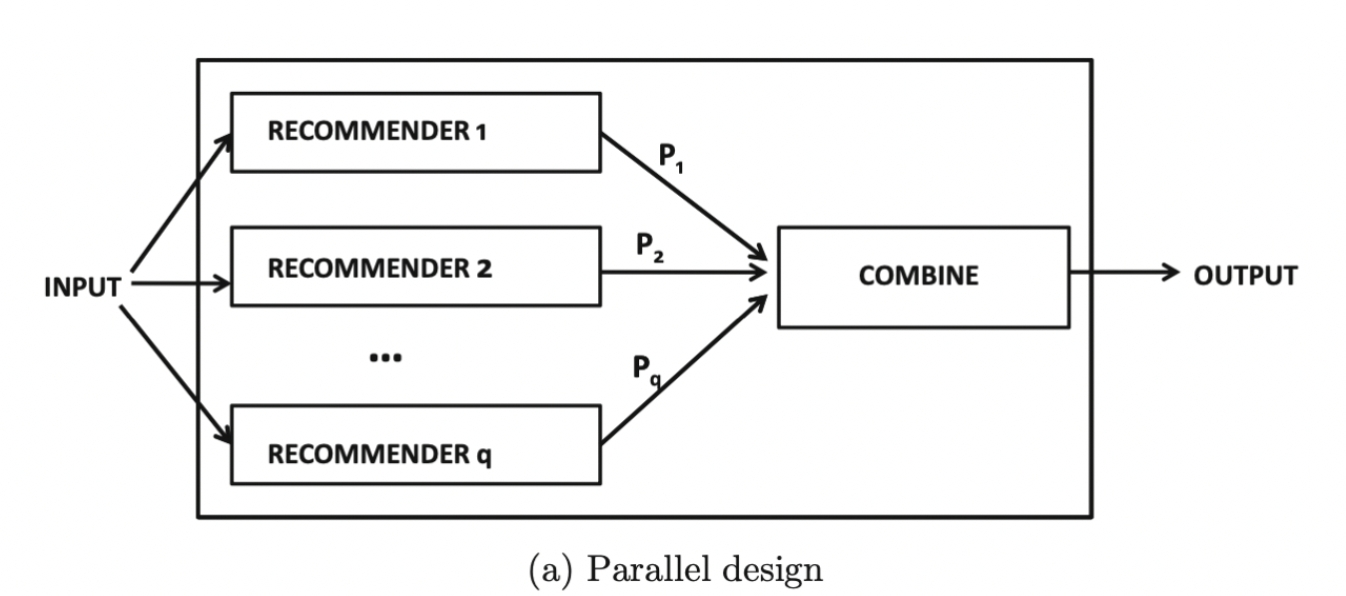
\includegraphics[scale = 0.5]{padesign}
% \caption{Parallel design of Hybrid Recommendation System}
% \centering
% \end{figure}
% \begin{figure}[ht]
% \centering
% 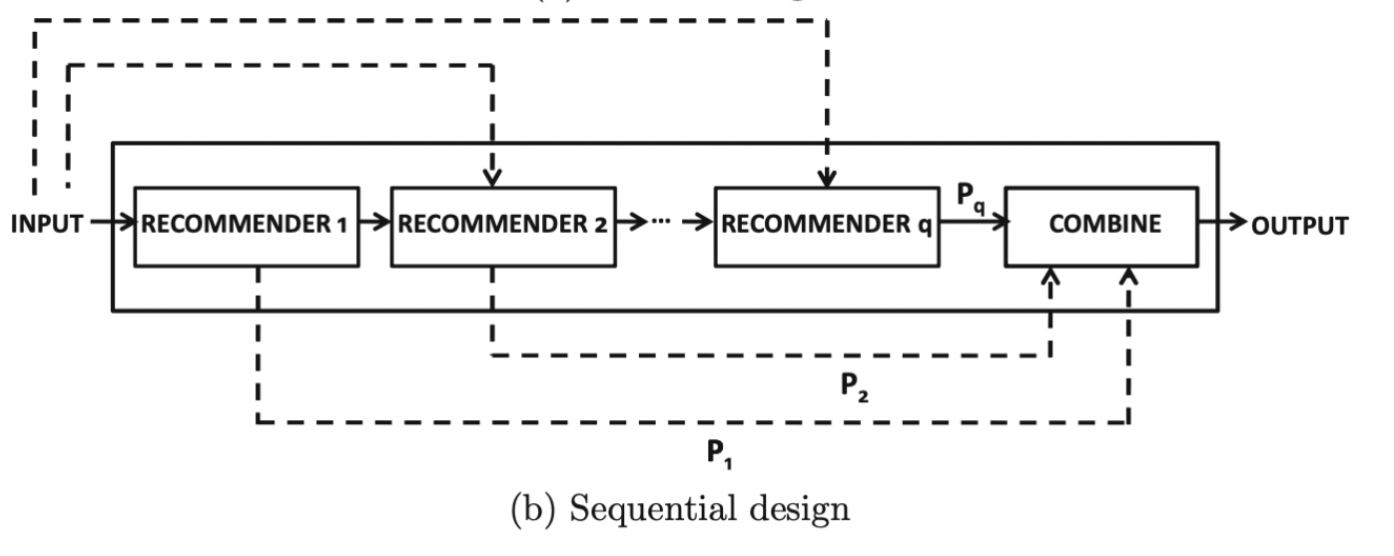
\includegraphics[scale = 0.5]{sedesign}
% \caption{Sequential design of Hybrid Recommendation System}
% \centering
% \end{figure}
\\\textbf{Advantages}
\\Hybrid systems combine different models to combat the disadvantages of one model with another. This overall reduces the weaknesses of using individual models and aids in generating more robust recommendations. This yields more robust and personalised recommendations for users.
\\\textbf{Disadvantages}
\\These types of models generally have high computational complexity and require a large database of ratings and other attributes to keep up to date. 
Without up-to-date metrics (user engagement, ratings, etc.), it is difficult to retrain and provide new recommendations with updated items and ratings from various users.

\section{Evaluation}
Identifying what defines a good recommendation is a problem many companies struggle with. This definition of “good” recommendations helps evaluate the performance of the recommender you built. 
A recommendation's quality can be assessed through various tactics that measure coverage and accuracy. 
Accuracy is the fraction of correct recommendations out of the offered possible suggestions. At the same time, coverage measures the fraction of objects in the search space for which the system can provide guidance. 
The evaluation method of a recommendation is solely dependent on the dataset and approach used to generate the request. 
Recommender systems share several conceptual similarities with the classification and regression modelling problem. 
In an ideal situation, we would want to see how real users react to recommendations and track metrics around the user to improve your recommendation request. However, this isn't easy to accomplish. 
Common standard statistical accuracy measures to evaluate the accuracy of a recommender are RMSD, MAE, and k fold cross-validation.

\subsection{K Fold Cross Validation}
This is one of the non-exhaustive validation methods, which means it does not compute all ways of splitting the original sample. K fold cross-validation can be used to infer the results of the model through accuracy metrics. We can create K many randomly assigned training and test sets by splitting the dataset, and each training set/fold is used to train on the recommendation system independently and then measure the accuracy of the resulting systems against the test set. Then we take the average accuracy score to see how well the recommendation system learns.
\\This method is beneficial to prevent your model from overfitting; however, it is a computationally extensive process.

\subsection{Mean Absolute Error (MAE)}
Mean absolute error represents the average absolute value of each error in rating prediction
\begin{equation*}
\text{MAE} = \frac{\sum^{i=n}_{i=1}|y_{i} - x_{i}|}{n}
\end{equation*}
where $y_{i} $ represents the prediction, $x_{i} $ is the true Value and $n$ is the total number of data points.

\subsection{Root Mean Square Deviation(RMSD)}
\begin{equation*}
\text{RMSD} = \sqrt{\frac{\sum^{i=N}_{i=1}(y_{i} - x_{i})^{2}}{N}}
\end{equation*}

\begin{itemize}
\item This is a similar metric to MAE but has a stronger penalty for when the prediction is very far from the true value, and a weaker penalty for when the prediction is closer to the true value
\item Taking the squares off the difference between true and predicted values instead of the sum of the absolute values. This ensures that the resulting value is always positive and is larger when the difference is high and smaller when the difference is low.
\end{itemize}


\section{Implementation}
\subsection{System Design}
We finally decided to design our recommendation system using a hybrid system shown in \autoref{hybridd}. The system consists of four sub-systems in parallel with each other, 
One of the sub-systems is built with content-based and model-based filtering connected in series.
\begin{figure}[ht]
    \centering
    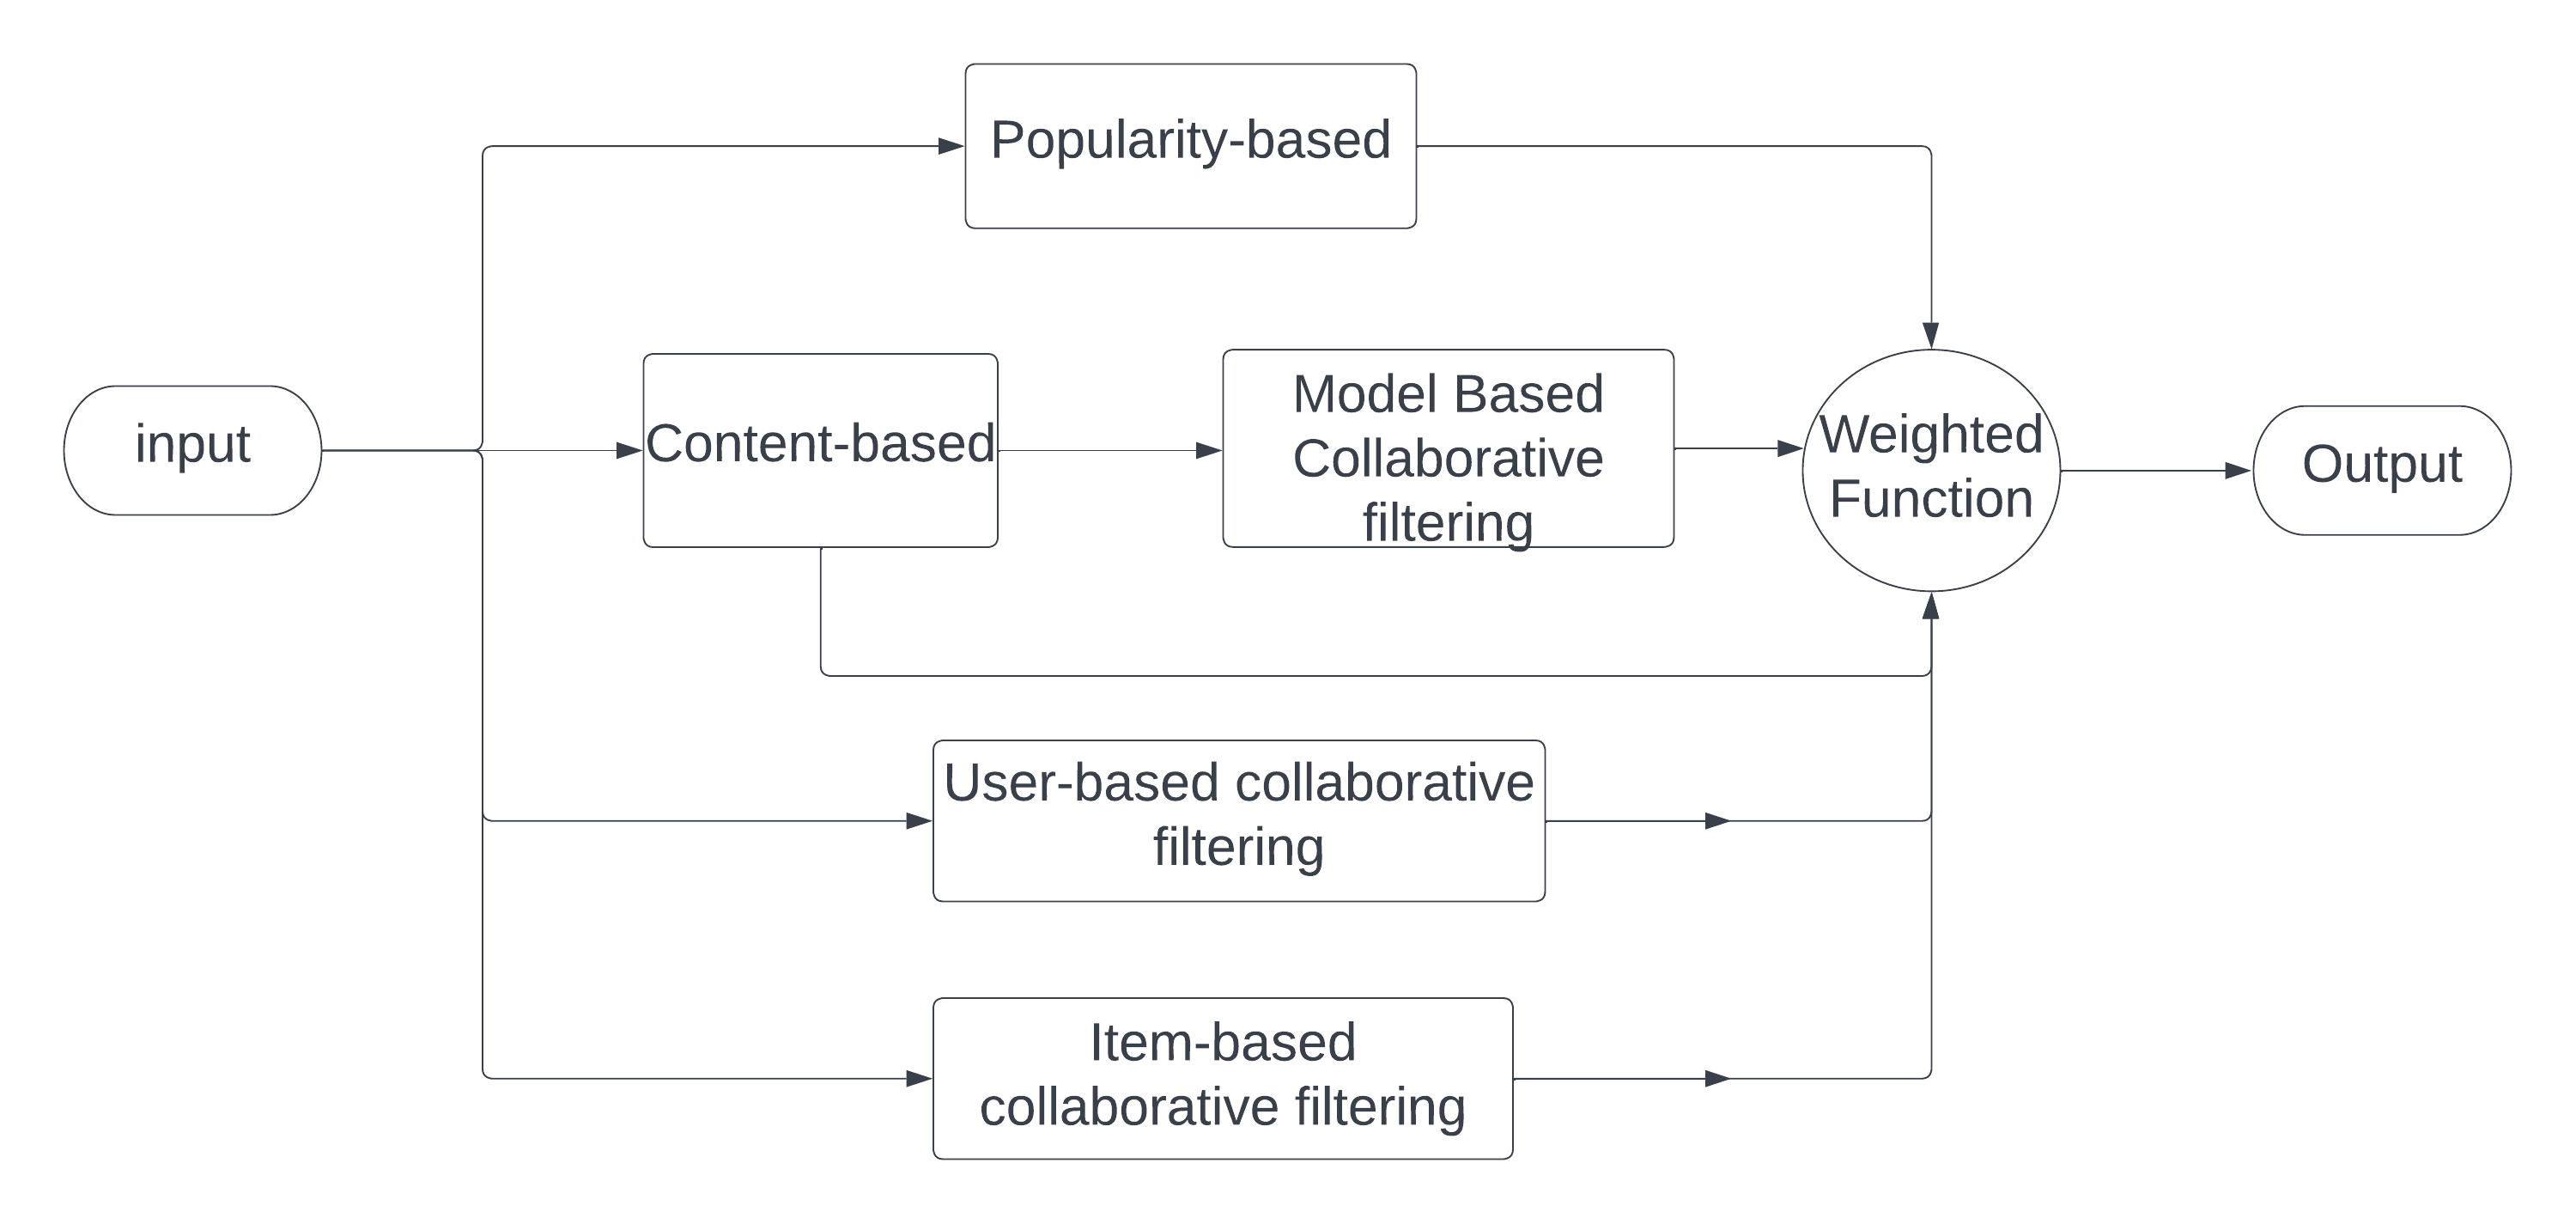
\includegraphics[scale = 0.15]{hybridd.png}
    \caption{Hybrid recommendation system design}
    \label{hybridd}
    \end{figure}
\\Firstly, the input, which is information gathered from our users, will be passed through the popularity based system to get the ratings for their popularity.
\\In addition, the input will be fed into a content-based system to have ratings based on the similarity between users' preferences and posts' features. 
We also pass the output after the content-based system through model-based collaborative filtering to solve the limitations in the last step, 
which is that the users' parameters vector can not be updated, and users will not be recommended the type of posts if they have not interacted with them before. 
\\Furthermore, the input will pass through the user-based and item-based collaborative filtering system in parallel with other systems 
to have the ratings of posts based on the analysis of group behaviours.
\\Finally, after we have ratings after each design, we pass all the results into a weighting function, where we give weights to each sub-system output and then apply a linear combination.
The weight coefficients are calculated based on the performance and reliability of the sub-systems.


